\section{Process Perspective}

\subsection{CI/CD Chain}

In order to introduce continuous integration and continuous deployment to the program, we used Github Actions, namely workflows. The project included several different workflows like provision and deploy as described in table \ref{tab:workflows}.

\begin{table}[H]
    \centering
    \begin{tabular}{|p{0.24\textwidth} | p{0.75\textwidth}|}
        \hline
        \textbf{Workflow file} & \textbf{Function}\\
        \hline
        \textit{AutomaticBuildRelease.Backend} &  Bumps the patch versioning of the \textit{MinitwitSimulatorAPI} project and creates a release on the github repository.\\
        \textit{AutomaticBuildRelease.Frontend} & Bumps the patch versioning of the \textit{Minitwit} project and creates a release on the github repository.\\
        \textit{WeeklyMinorRelease} & Bumps the minor version of the entire program and creates a release each Thursday at 20:00 UTC.\\
        \textit{Linters-and\_Formatter} & Runs Hadolint, Pre-commit, and the dotnet-format linter, when a PR is created, modified, and reopened.\\
        \textit{Testing} & Runs all tests on the infrastructure, the frontend, and the backend, when a PR is created, modified, and reopened.\\
        \textit{Provision-and-Deploy} & Provision and deploy swarm and observability servers using Ansible for server provision and Pulumi for infrastructure as code, on pushes to main.\\
        \textit{latex-build} & Creates a report PDF when changes have been made to the report.\\
        \hline
    \end{tabular}
    \caption{The function of the workflows}
    \label{tab:workflows}
\end{table}

Figure \ref{fig:workflows} vizualizes the development pipeline all the way from writing code to production. This includes running precommit to check for formatting to passing both UI and integrations tests as well as building and deploying.

\begin{figure}[H]
    \centering
    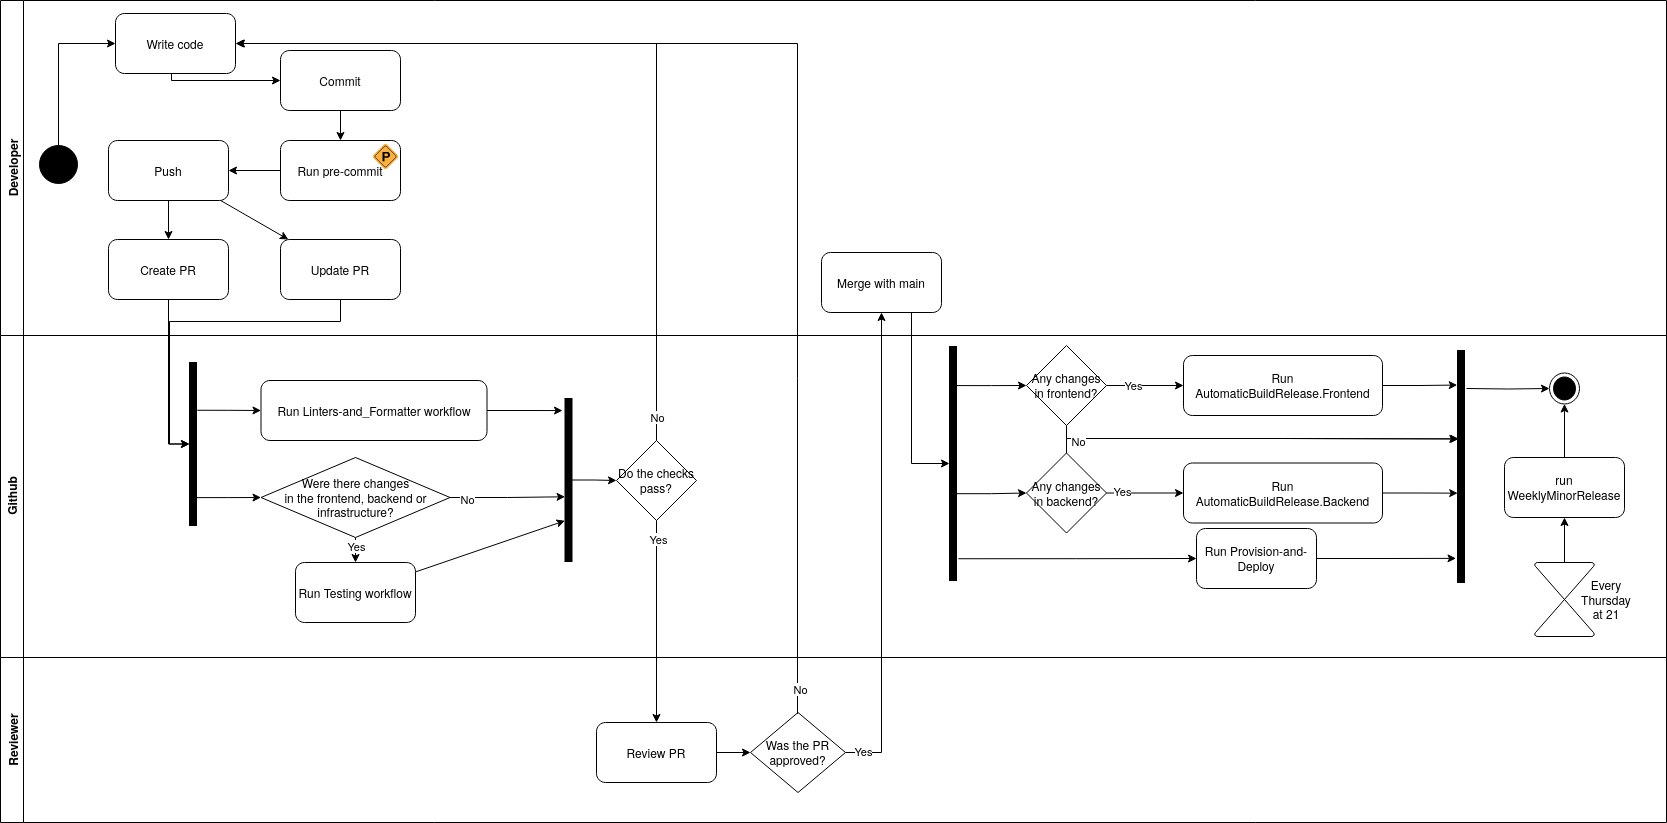
\includegraphics[angle=270, scale=0.37]{Github-Actions.png}
    \caption{Activity diagram showcasing the workflows interacting }
    \label{fig:workflows}
\end{figure}

\subsection{Monitoring and logging}
For monitoring we use Grafana. We export metrics by using OpenTelemetry and collect the metrics via Prometheus and lastly push them to Grafana. Our board shows requests duration, errors rate, top 10 unhandled exception endpoints and more (for visualization of the board, see appendix \ref{appendix:grafana}). We have used the board to get an overview of where to put our focus, ie. which endpoints to improve, which errors to fix, etc. Moreover, we are gaining insights into the health of the system and get an impression of how the backend and frontend handle the requests.

For logging, we use Grafana and Loki. It seemed natural to continue our work with Grafana in order to keep the system setup as simple as possible. The logs are divided into Information, Warning, Debug and Error. All logging statements are placed in the controllers, such that we have information about the users' whereabouts in the system. For example, we log when a user logins whether successful or not.

\subsection{Security Assessment}
Based on our security assessment (see appendix \ref{appendix:securityassesment}), we constructed the following risk matrix:
\begin{figure}[H]
    \centering
    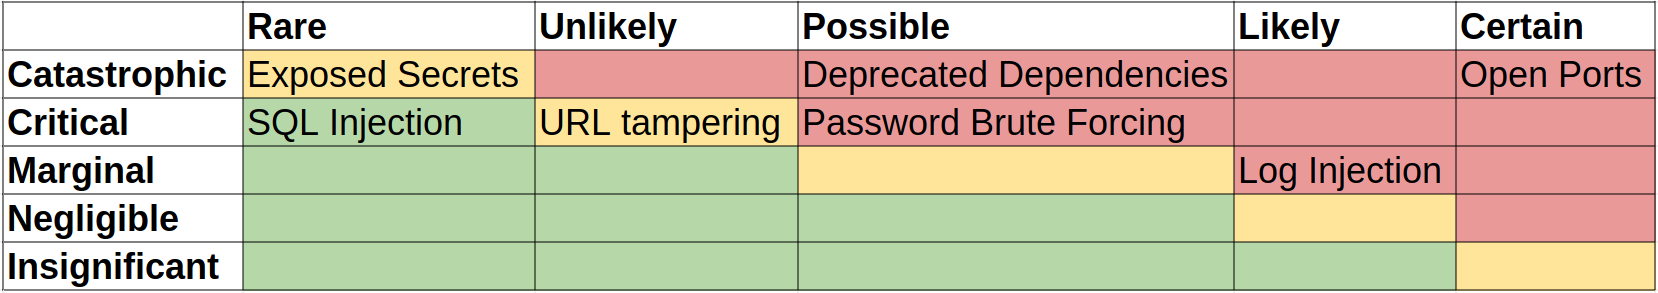
\includegraphics[width=1\linewidth]{images/risk-matrix.png}
    \caption{Risk matrix from security assessment}
    \label{fig:enter-label}
\end{figure}
We decided to focus on the scenarios in the red zone, as they would be the cause of most damage. Due to the team not having enough knowledge about how the simulator worked in regards to creating users and logging in, we did not move further with the \textit{Password Brute Forcing} scenario. However, possible solutions could be to incorporate 2FA, password requirements and time-out limitation for an actual system in production.

For \textit{Log Injection}, we made sure to sanitize user inputs, as they previously were put directly into the log, which could be exploited to hide ill-intentioned actions. We thereby hardened the system against injection attacks.

With \textit{Depricated Dependencies}, we chose to integrate the tool \textit{dependabot} into our CI/CD pipeline to watch out for outdated dependencies in our main repository. This helps us ensure that an adversary is not able to take advantage of the team not being aware of vulnerabilities in variuos of the used tools.

\textit{Open Ports} was deemed the biggest risk, as this was most likely the reason for us being hacked, which we have written about in further details in section \ref{section_hacked}. We used the tool \textit{nmap} to scan the IP address of our application and check for open ports, which showed the following:
\begin{figure}[H]
    \centering
    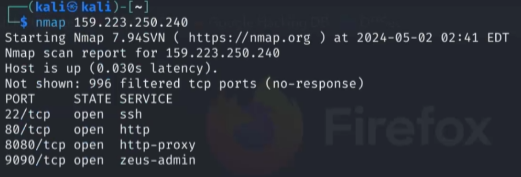
\includegraphics[width=1\linewidth]{images/nmap.png}
    \caption{Open ports found by nmap}
    \label{fig:matrix}
\end{figure}
We tried to close port 9090, which was used for Prometheus, but it was unclear if we were successful as \textit{nmap} kept showing the port as open, despite seeing the firewall configuration say otherwise on the server itself. This was likely caused by Docker bypassing our firewall, which was handled by the Ansible ufw module, through IP tables.

\subsection{Scaling}
We use horizontal scaling, as we wanted a more resilient application and limit downtime when deploying. We settled on Docker Swarm over building a custom load balancer or adopting Kubernetes, primarily due to its simplicity and compatibility with the existing system setup. To implement Docker swarm we created a new server in our system and added a manager and a worker node to the swarm.

When attempting to scale by adding another frontend replica, we encountered challenges. In order for the two replicas to work together we needed to handle distributed sessions to remember who is logged in even though the frontend replica is switched. However, we did not succeed in this (we refer to week 11 in the log in appendix \ref{appendix_log}), which is the reason why we only have a single frontend replica.

For the update strategy we went with rolling updates because it is the default update strategy for Docker Swarm.
